\section{Description}
The product can be logically divided into two applications -- server side  and client side.
Each application will be used by different kind users and for better distinguishing of all terms we feel need to define them.

\section{Definitions}
In this section there will be defined and described actors in requirements to avoid misunderstandings. Since our customer namely specified the domain that we should focus on we named the actors as follows.

\paragraph{User} is a participant of concert who wants to actively take part in show and he can download client application.

\paragraph{Concert Manager} or simply \textbf{Manager} is a person who controls what media should be played on screen made from mobile phone's of users. 
He can also manage other general settings.

\paragraph{Client} or \textbf{Client side} is an application controlled by user and provides him opportunity to be part of the screen by displaying figures on his mobile.

\paragraph{Server} or \textbf{Server side} is and application controlled by manager and provides him opportunity to change the media displayed on screen.

\section{Business Requirements}
\subsection{Functional}

\begin{table*}[!h]\centering
\caption{List of all chapters and short description. }
\label{tab:req_func}
\def\arraystretch{1.3}
\begin{tabularx}{\textwidth}{llX}
\toprule[1mm]
\textbf{ID} & Name & Description\\
\midrule
\phantomsection\label{req_F1}\textbf{F1} & Client behavior & Client must be able to receive commands from the server and display color according to the instructions.\\
\textbf{F2} & More servers & An user can specify to which server (concert stage) he wants to connect.\\
\textbf{F3} & Localization & Server must be able to detect mobile device's positions using image processing.\\
\textbf{F4} & Core & Server should be able to display media through a few (a least 3) mobile phones' screens.\\
\textbf{F5} & Media selection & A manager can choose which media should be played on screen made from mobile phones' screens.\\
\textbf{F6} & Attendance & Number of connected devices to server must be displayed in server application. \\

\bottomrule[1mm]

\end{tabularx}
\end{table*}

\subsection{Non-functional}

\begin{table*}[!h]\centering
\caption{List of all chapters and short description. }
\label{tab:req_nonfunc}
\def\arraystretch{1.3}
\begin{tabularx}{\textwidth}{llX}
\toprule[1mm]
\textbf{ID} & Name & Description\\
\midrule
\textbf{N1} & Server-client architecture & Application must work as a server and client architecture.\\
\textbf{N2} & Platform & Audience application must work on at least one mobile platform.\\
\textbf{N3} & Deployment & Application must be deployed to relevant mobile application store.\\
\textbf{N4} & Scalability & The application must be scalable - it must work with different count of mobile phones.\\
\textbf{N5} & Generality & The application must be prepared for future using outside of rock concert domain.\\
\textbf{N6} & Delivery & Final product must be finished until 21st of November 2013 and presented to the committee and the customer.\\
\bottomrule[1mm]

\end{tabularx}
\end{table*}
\section{Use case diagram}
In the figure bellow is shown use case diagram \ref{img:usecase} of the whole system.

\begin{figure}[h]
    \begin{center}
    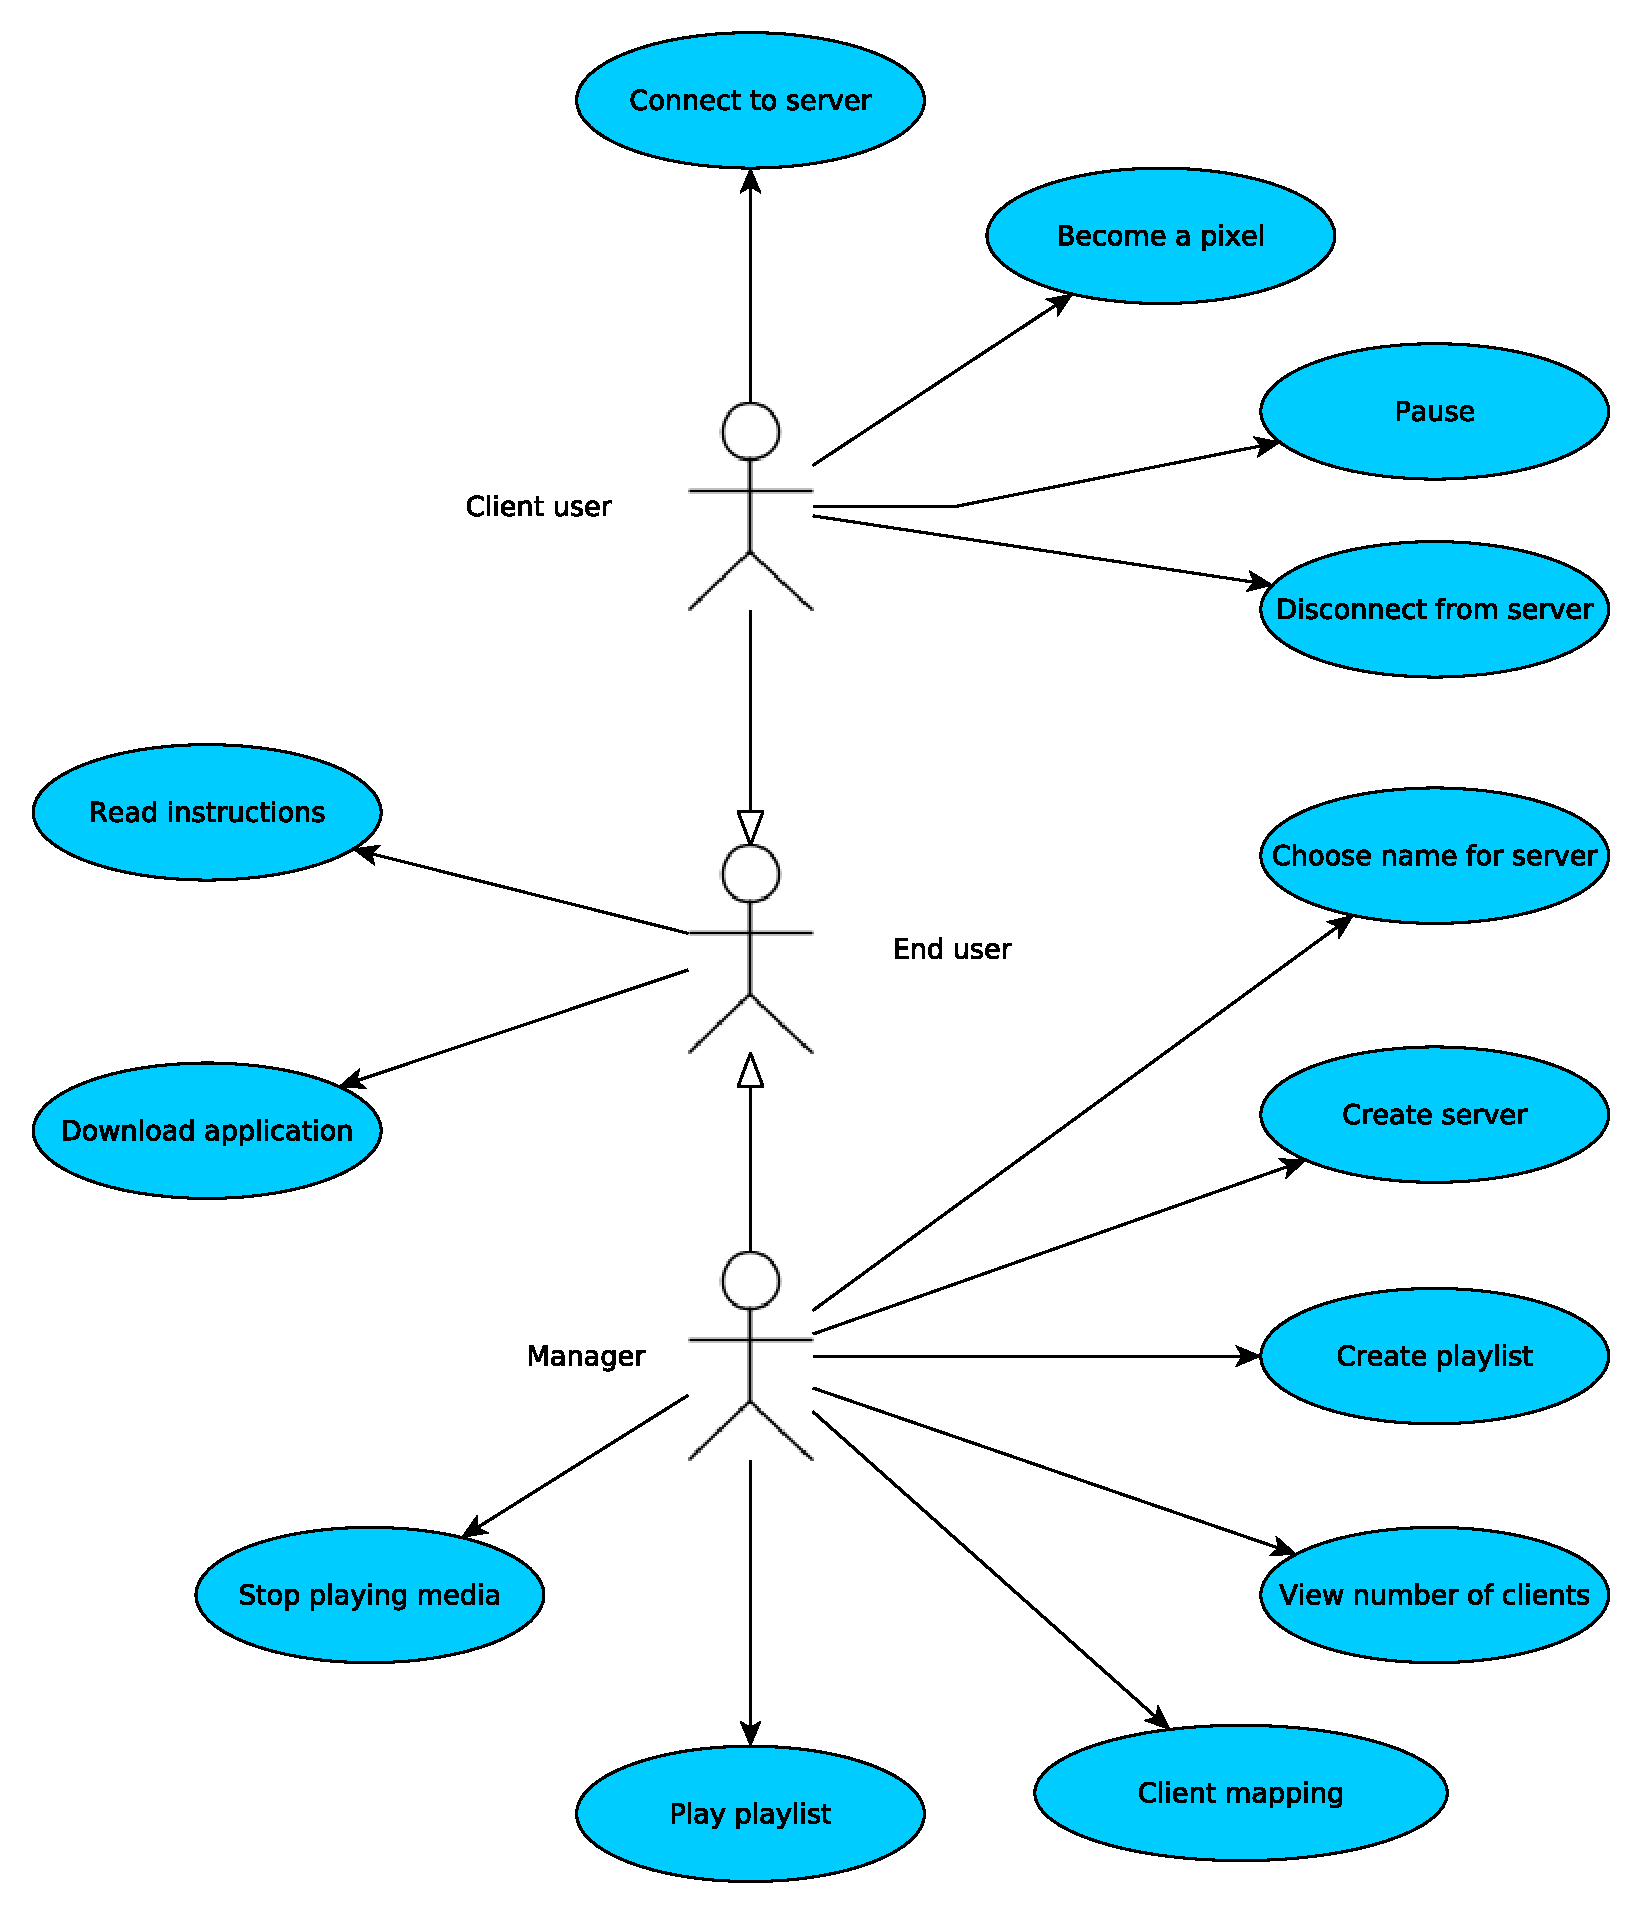
\includegraphics[scale=0.4]{images/usecase.pdf}
    \caption{Use case diagram for both actors User and Manager.}
    \label{img:usecase}
    \end{center}
\end{figure}

%\begin{table*}[!h]
%	\def\arraystretch{1.25}
%	\caption{User stories selected for Sprint 0. }
%	\label{tab:usecase1}
%	
%	\begin{tabular}{p{\textwidth}}
%		\toprule[1mm]
%		\textbf{Use Case detail: Create playlist} \\
%		\midrule	
%		Actors: Manager \\
%		Conditions:
%		
%		\begin{enumerate}
%			\item Manager had created server.
%		\end{enumerate}
%		\bottomrule[1mm]
%	\end{tabular}
%\end{table*}

\section{Summary}
